% !TEX TS-program = xelatex


\documentclass[a4paper,14pt]{extarticle}

% Include settings from setting.tex
\input{setting.tex}

\geometry{a4paper, margin=1in}
\graphicspath{{img/}}

\newcommand{\assignNum}{3} %change the number of the assignment here
\author{مرتضی ملکی‌نژاد شوشتری} %change your name here
\newcommand{\SNum}{810104256} %change your SID here
\date{\today}
\title{تمرین \assignNum}

\begin{document}
\pagenumbering{gobble}
\maketitle
\newpage
\tableofcontents

\newpage
\listoffigures

\newpage
\listoftables

\newpage
\pagenumbering{arabic}

\section{چکیده}

\newpage
\setcounterref{section}{0}
\lr{\section{Perceptron}}
\subsection{}
{
\centering
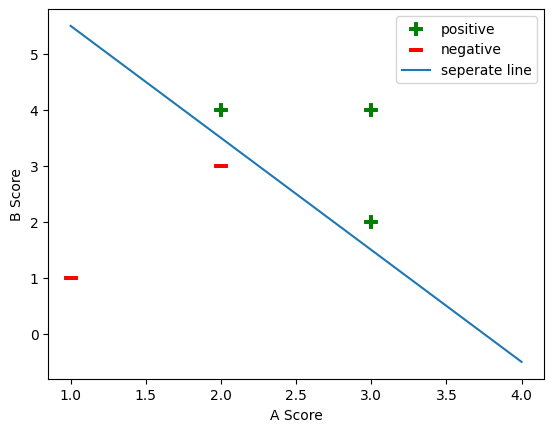
\includegraphics[width=0.8\textwidth]{img/q1_1.png}
\captionof{figure}{نمودار نقاط باتوجه به امتیازها. داده‌ها بصورت خطی جداپذیر هستند، یکی از این خط‌ها رسم شده است.}
}
\subsection{}
مقدار 
\lr{learning rate}
برابر
$0.05$
درنظر گرفته شده است.
\begin{table}[h]
	\centering
	\caption{خروجی \lr{Perceptron} در هر گام}
	\begin{latin}
	\begin{tabular}{|c|c|c|c|}
		\hline
		Step & Weight & Score & Correct? \\
		\hline
		1 & [-1, 0, 0] & -1.1 + 0.1 + 0.1 = -1 & yes \\
		2 & [-1, 0, 0] &  -1 & no \\
		3 & [-0.95, 0.15, 0.1] & -0.25  & no \\
		4 & [-0.9   0.25  0.3 ] & 1.05 &yes \\
		5 & [-0.9   0.25  0.3 ] & 0.5 & no \\
		\hline
	\end{tabular}
		\end{latin}
\end{table}
\subsection{}
باتوجه به نمودار کشیده شده، هنوز خط جداسازی به طور کامل یادگرفته نشده است.
{
	\centering
	
\includegraphics[width=0.8\textwidth]{img/q1_2.png}
	\captionof{figure}{نمایش خط یادگرفته شده در مرحله ۲}
}
البته اگر همین پرسپترون به دفعات بیشتری آموزش ببیند می‌تواند این داده را بصورت کامل جداسازی کند. 

{
	\centering
	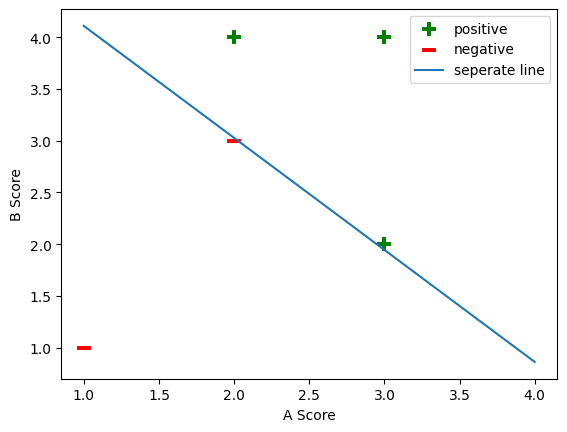
\includegraphics[width=0.8\textwidth]{img/q1_3.png}
	\captionof{figure}{خروجی پرسپترون پس از ۵۰ بار یادگیری و با ضریب یادگیری $0.005$. مدل موفق شده خطی را بیابد که دسته‌ها را بطور کامل جدا کرده است.}
}
\subsection{}
در هر مورد باید بررسی کرد که دسته‌ها بصورت خطی جداپذیر هستند یا خیر. یعنی ایا وزنی هست که مدل با رسیدن به آن ها بتواند با علامت \lr{score} دسته‌ها را پیش‌بینی بکند یا خیر. اگر وجود داشته باشد یعنی مدل می‌تواند (و ابر متغیرها باید درست تنظیم شوند) و اگر نباشد مدل با هیچ وزنی نمی‌تواند دسته‌ها را جدا کند.
\lr{\subsubsection{a}}
بله. درواقع مدل باید بتواند به وزن 
$[-8, 1, 1]$
برسد.
\lr{\subsubsection{b}}
این داده بصورت خطی جداپذیر نیست (درواقع ناحیه بین دو خط در صفحه است) و مدل نمی‌تواند این را بصورت کامل یاد بگیرد. 
\lr{\subsubsection{c}}
این مورد نیز خطی جداپذیر نیست (درواقع خود یک خط است) و مدل نمی‌تواند این را یاد بگیرد.
\newpage
\lr{\section{Neural Networks: Representation}}
ابتدا هر شبکه بررسی می‌شود:
\begin{itemize}
	\item 
	\textbf{
	\lr{G1}}
	این شبکه چون عنصر غیر خطی ندارد فقط قادر است توابع خطی را پیش‌بینی کند. همچنین چون عنصر بایاس ندارد،‌خط باید حتما از مبدا بگذرد.
	\item 
	\textbf{
		\lr{G2}}
		مشابه قسمت قبل این شبکه نیز عنصر غیر خطی ندارد و نمی‌تواند توابع غیرخطی را پیش‌بینی کند. ولی چون بایاس دارد، لزومی ندارد خط از مبدا بگذرد.
		\item 
		\textbf{
			\lr{G3}}
			با اینکه به این شبکه عنصر غیر خطی 
			\lr{relu}
			اضافه شده است،‌ولی 
			
			\lr{relu}
			بدون بایاس و با تنها یک بایاس ضعیف است. در اینجا عملا وزن‌های گره دوم تاثیری ندارند (تنها این قابلیت را به مدل می‌دهند که خروجی منفی بدهد.) 
			\item 
			\textbf{
				\lr{G4}}
				خروجی این قسمت بعد از اعمال 
				\lr{relu}
				یک خط شکسته شبیه به خود تابع 
				\lr{relu} 
				است با این تفاوت که نقطه شکست روی صفر نیست و با مقدار 
				$w_1$
				و
				$b_1$
				تعریف می‌شود. 
				گره دوم ولی تاثیر زیادی ندارد و صرفا شیب خط را (در جایی که خود تابع بخاطر اعمال \lr{relu} صفر نشده) عوض می‌کند. یعنی عملا قابلیت جدیدی نمی‌دهد (مشابه قسمت ۳ تنها فایده این گره این است که تابع می‌تواند مقادیر منفی را نیز خروجی دهد.)
				\item 
				\textbf{
					\lr{G5}}
					این تابع بسیار مشابه قسمت ۴ است و تنها یک بایاس به آن اضافه شده است. یعنی می‌تواند هر خط شکسته‌ای که یک قسمت آن موازی محور 
					\lr{x}
					ها هست را پیش‌بینی کند.
		
\end{itemize}
شبکه‌های دوبعدی عملا ترکیب دوتا از این شبکه‌های تک بعدی هستند. در موارد غیر خطی قاعده مهم این است که اگر نقاط شکست از تعداد توابعی که 
\lr{relu}
روی آن‌ها اعمال شده است بیشتر باشند نمی‌توان آن ها را پیش‌بینی کرد.
\lr{\subsection{a1}}
این یک تابع خطی گذرنده از مبدا است و همه شبکه‌ها می‌توانند آن را پیش‌بینی کنند.
\lr{\subsection{a2}}
این یک تابع خطی است که از مبدا نمی‌گذرد و به غیر از 
\lr{G1}
و 
\lr{H1}
سایر شبکه‌ها می‌توانند آن را پیش‌بینی کنند.
\lr{\subsection{b1}}
این یک تابع شکسته است که هر دو تکه آن شیب غیر صفر دارند. برای همین از شبکه‌های یک بعدی هیچ کدام نمی‌توانند آن را پیش‌بینی کنند ولی در شبکه‌های دو بعدی، هر مسیر می‌تواند یک تکه را یاد بگیرد (و تکه دیگر صفر باشد) و سپس این دو لایه با هم جمع می‌شوند 
چون نقطه شکست روی مبدا است نیازی به بایاس نیست پس یعنی شبکه‌های 
\lr{H3, H4}
و 
\lr{H5}
می‌توانند این تابع را یاد بگیرند. 
\lr{\subsection{b2}}
خروجی 
\lr{relu}
از یک طرف شیب غیر صفر دارد ولی این شکل از هر دو طرف شیب صفر دارد. برای خروچی گرفتن همچنین شکلی حداقل به دو 
\lr{relu}
متوالی
نیاز است. پس هیچ یک از شبکه‌ها نمی‌توانند این تابع را یاد بگیرند. تعداد نقاط شکست برابر ۳ است یعنی شبکه‌های دوبعدی نیز نمی‌توانند بطور دقیق همه تابع را بسازند.
\lr{\subsection{c1}}
با هیچ یک از شبکه‌های یک بعدی نمی‌توان ولی با شبکه دو بعدی می‌توان صرفا باید یکی از قسمت‌هایی که شیب صفر دارند را با خنثی کردن ابعاد خروجی گرفت. پس یعنی نیاز به شبکه‌هایی داریم که پس از یک لایه 
\lr{relu}
بتوانند خروجی های تابع شکسته با \lr{bias}
بدهند. 
یعنی شبکه‌های 
\lr{H4}
و 
\lr{H5}
.
\lr{\subsection{c2}}
تابع دو نقطه شکست دارد. نکته مهم این است که با این که این تابع عملا ترکیب سه خط است ولی شیب قسمت وسط برابر جمع شیب دوتکه دیگر است. پس یعنی می‌توان با دوتابع شکسته آن را ساخت. همچنین چون تابع شیفت یافته است باید در لایه پس از \lr{relu} بایاس داشت پس یعنی فقط مدل 
\lr{H5}
می‌تواند این تابع را بسازد.

{
\centering
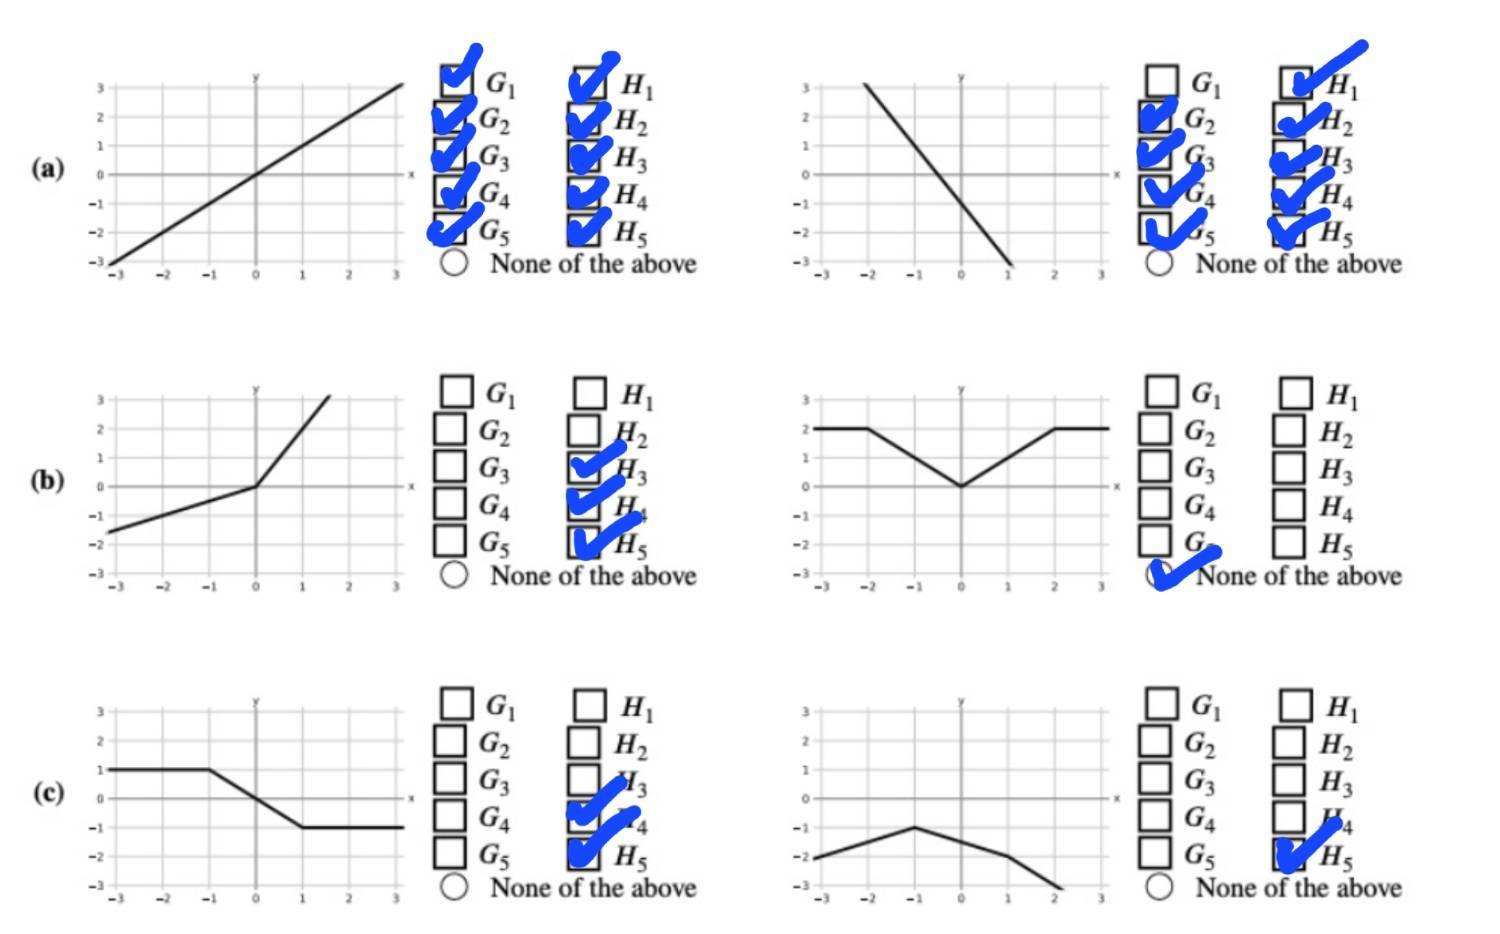
\includegraphics[width=0.8\textwidth]{img/q2.jpg}
\captionof{figure}{هر تابع را چه مدل‌هایی می‌توانند یاد بگیرند.}
}
\newpage
\lr{\section{Neural Networks: Forward and Backward Propagation}}
\subsection{}
\begin{table}[h]
	\centering
	\caption{ابعاد هر پارامتر در حالت معمولی}
	\begin{latin}
		\begin{tabular}{|c|c|}
			\hline
			Name & Dimension \\
			\hline
			$W_1$ & $D_{a_1} \times D_x$ \\
			$b_1$ & $D_{a_1} \times 1$ \\
			$W_2$ & $1 \times D_{a_1}$ \\
			$b_2$ & $1 \times 1$ \\
			\hline
		\end{tabular}
	\end{latin}
\end{table}
در حالت \lr{vectorize} فرمول قسمت 
\lr{z}
به این صورت در می‌آید:
$
z = XW + b
$
\begin{table}[h]
	\centering
	\caption{ابعاد هر پارامتر در حالت \lr{vectorize}}
	\begin{latin}
		\begin{tabular}{|c|c|}
			\hline
			Name & Dimension \\
			\hline
			$X$ & $n \times D_x$ \\
			$Y$ & $n \times 1$ \\
			$W_1$ & $D_x \times D_{a_1}$\\
			$b_1$ & $ n \times  D_{a_1}$\\
			$W_2$ & $D_{a_1} \times 1$\\
			$b_1$ & $ n \times  1$\\
			\hline
		\end{tabular}
	\end{latin}
\end{table}
\subsection{}
چون نمونه‌ها از هم مستقل هستند عملا باید مقدار مشتق تابع 
$
\cfrac{-1}{m}L^{(i)}
$
را نسبت به 
$
\hat{y}^{(i)}
$
حساب کرد. پس داریم:
\begin{latin}
	~\\
	$
	\cfrac{\partial J}{\partial \hat{y}^{(i)}} = \cfrac{-1}{m} *\cfrac{\partial (
		y^{(i)} log\ \hat{y}^{(i)} + (1 - y^{(i)})log\ (1 - \hat{y}^{(i)})
		)}{\partial \hat{y}^{(i)}}
		\\
		=
		\cfrac{-1}{m}
		*
		(
		\cfrac{y^{(i)} }{\hat{y}^{(i)}}
		+
		\cfrac{(y^{(i)} - 1)}{1 - \hat{y}^{(i)}}
		)
	$
\end{latin}
برای همه نمونه‌ها این مقدار جمع می‌شود پس داریم:
\begin{latin}
	$
	\cfrac{\partial J}{\partial \hat{y}} = \cfrac{1}{m } \sum\limits_{i = 1}^m (\cfrac{1 - y^{(i)}}{1 - \hat{y}^{(i)}} - \cfrac{y^{(i)}}{\hat{y}^{(i)}})
	$
\end{latin}
در کسرها اگر حالت صفر صفرم رخ داد، جواب صفر است زیرا در صورت صفر مطلق رخ می‌دهد و در مخرج صفر حدی.

\subsection{}
برابر با مشتق تابع سیگوئید برحسب 
\lr{z}
می‌شود. 
\begin{latin}
	$
	\cfrac{\partial \hat{y}}{\partial z_2^{(i)}} = \cfrac{e^{-z_2^{(i)}}}{(1 + e^{-z_2^{(i)}})^2}
	$
\end{latin}
\subsection{}
\lr{$z_2$}
یک تابع خطی برحسب 
\lr{$a_1$}
است که وزن آن 
$W_2$
است. پس یعنی مقدار 
$\delta_3^{(i)}$
برابر با 
$W_2$
است.
\subsection{}
مشتق تابع 
\lr{relu}
یک تابع بصورت زیر است:
\begin{latin}
	$
	U(x) = \left[
	\right]
	$
\end{latin}
\end{document}